\documentclass{article}
\usepackage{graphicx}

\title{Laporan Database 2}
\author{A.Iqham Syahihafiat (1184032)}
\date{02 November 2019}

\begin{document}

\maketitle

\section{Langkah-Langkah Pembuatan Sistem Informasi di Oracle Apex:}
\begin{enumerate}
    \item Langkah pertama yaitu membuka link https://apex.oracle.com/en/.dan selanjutnya klik sign in.
  \begin{center}
    
\includegraphics[width=.8\textwidth]{tb.PNG}
\end{center}
    \item isi data kita.. seperti dibawa ini.
    \begin{center}
    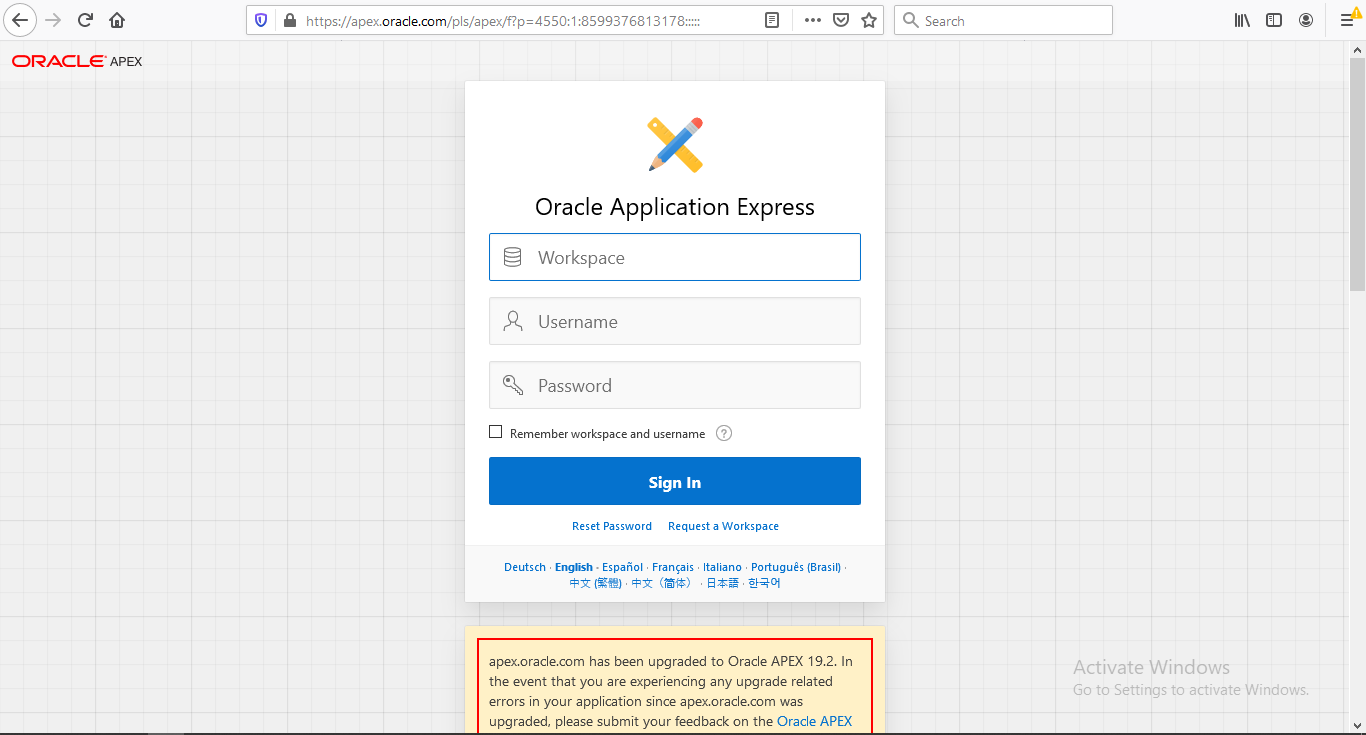
\includegraphics[width=.8\textwidth]{tb2.PNG}
\end{center}
    \item Untuk membuat aplikasi kita pilih app builder
    \begin{center}
    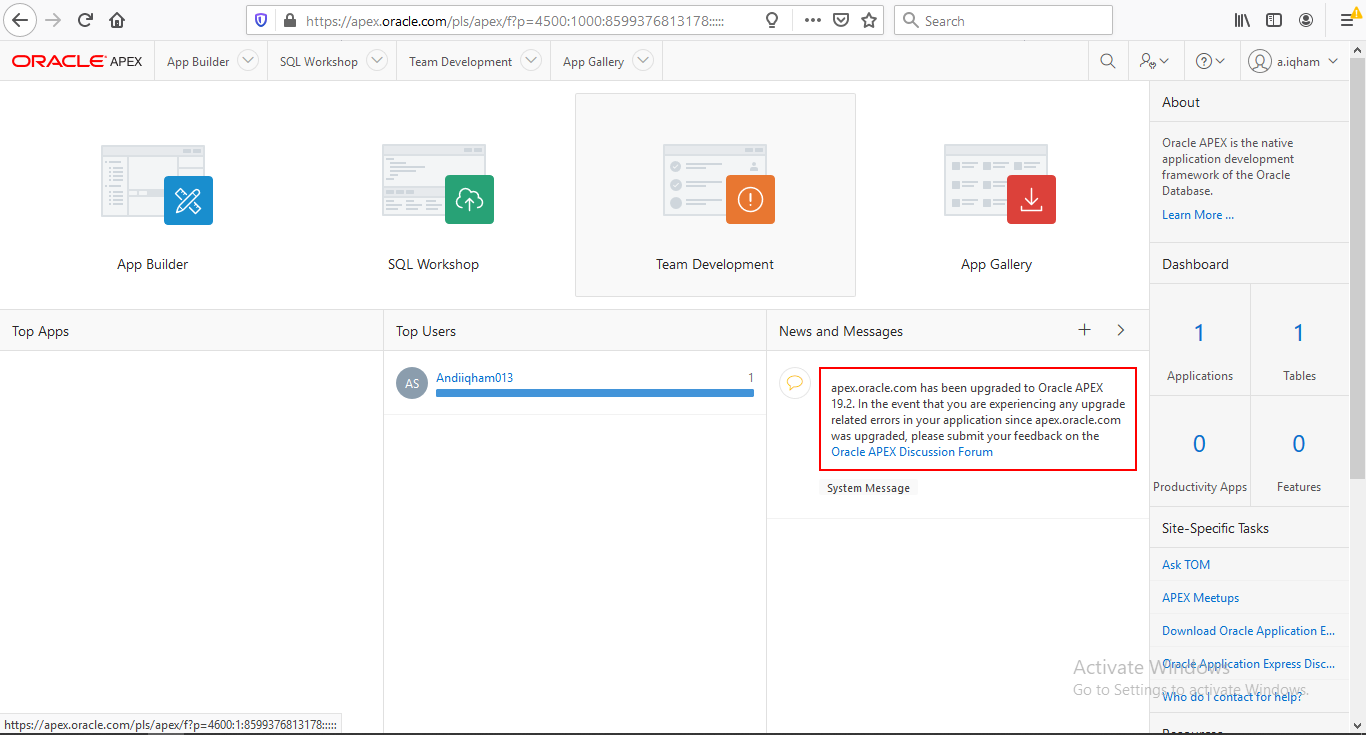
\includegraphics[width=.8\textwidth]{tb3.PNG}
\end{center}
    \item Untuk memasukkan data dari komputer kita,kita pilih create.
    \begin{center}
    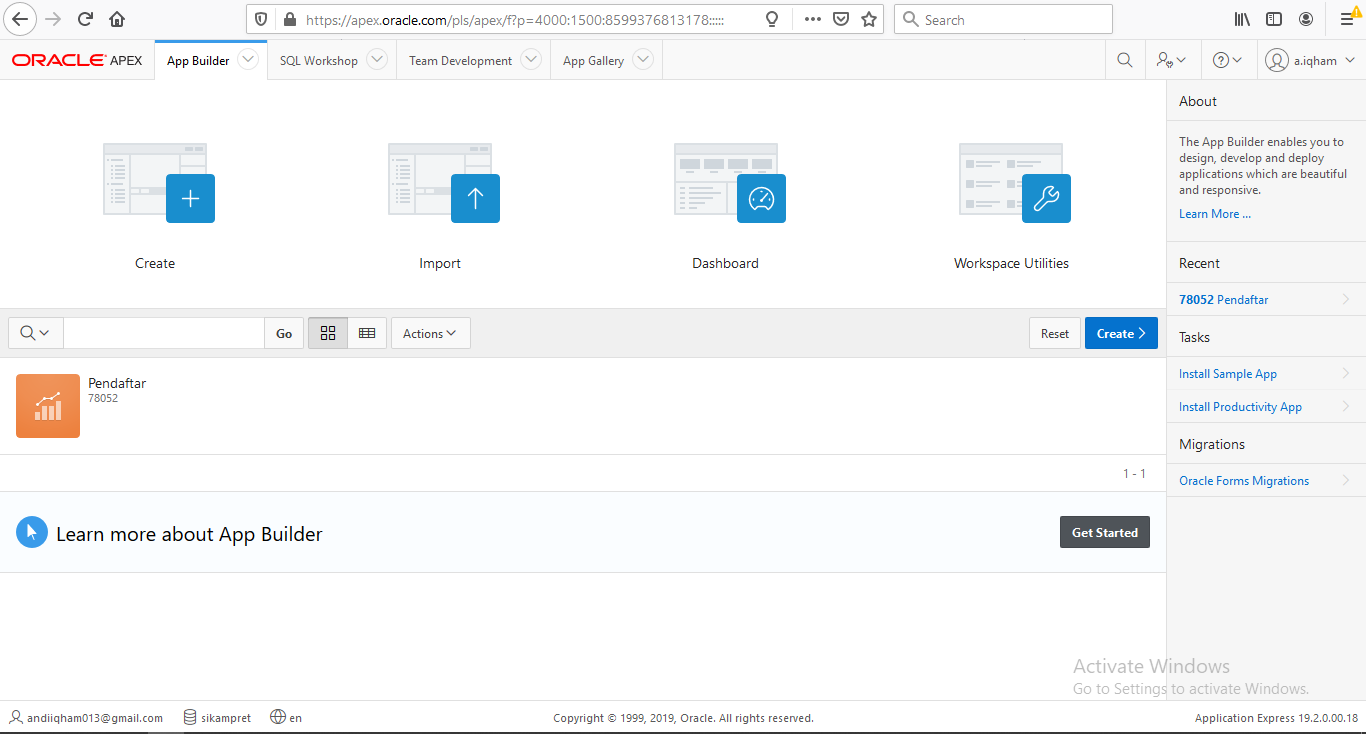
\includegraphics[width=.8\textwidth]{tb4.PNG}
\end{center}
    \item untuk memasukkan data kita pilih From a file ,jika sudah kita pilih data mahasiswa yang ingin dimasukkan.
    \begin{center}
    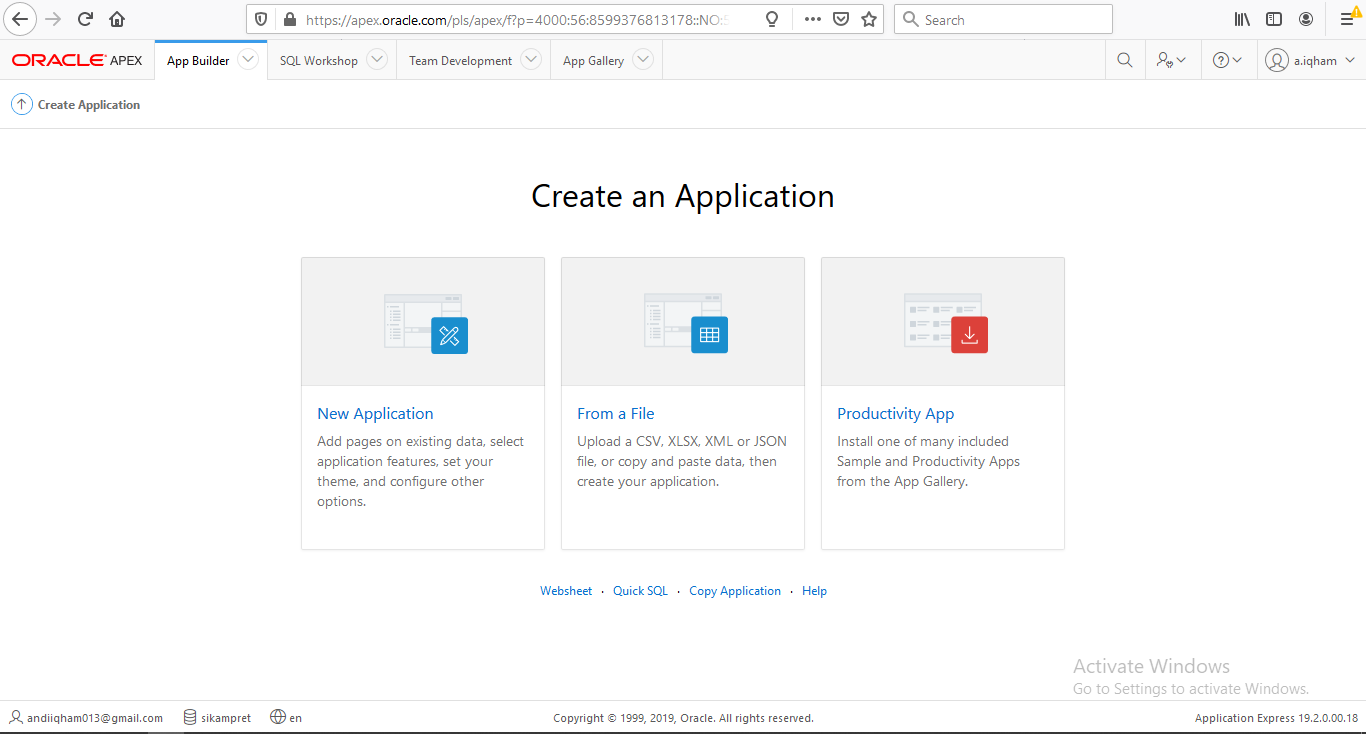
\includegraphics[width=.8\textwidth]{tb5.PNG}
\end{center}
    \item Jika data telah berhasil di input maka akan tampil seperti ini..
    \begin{center}
    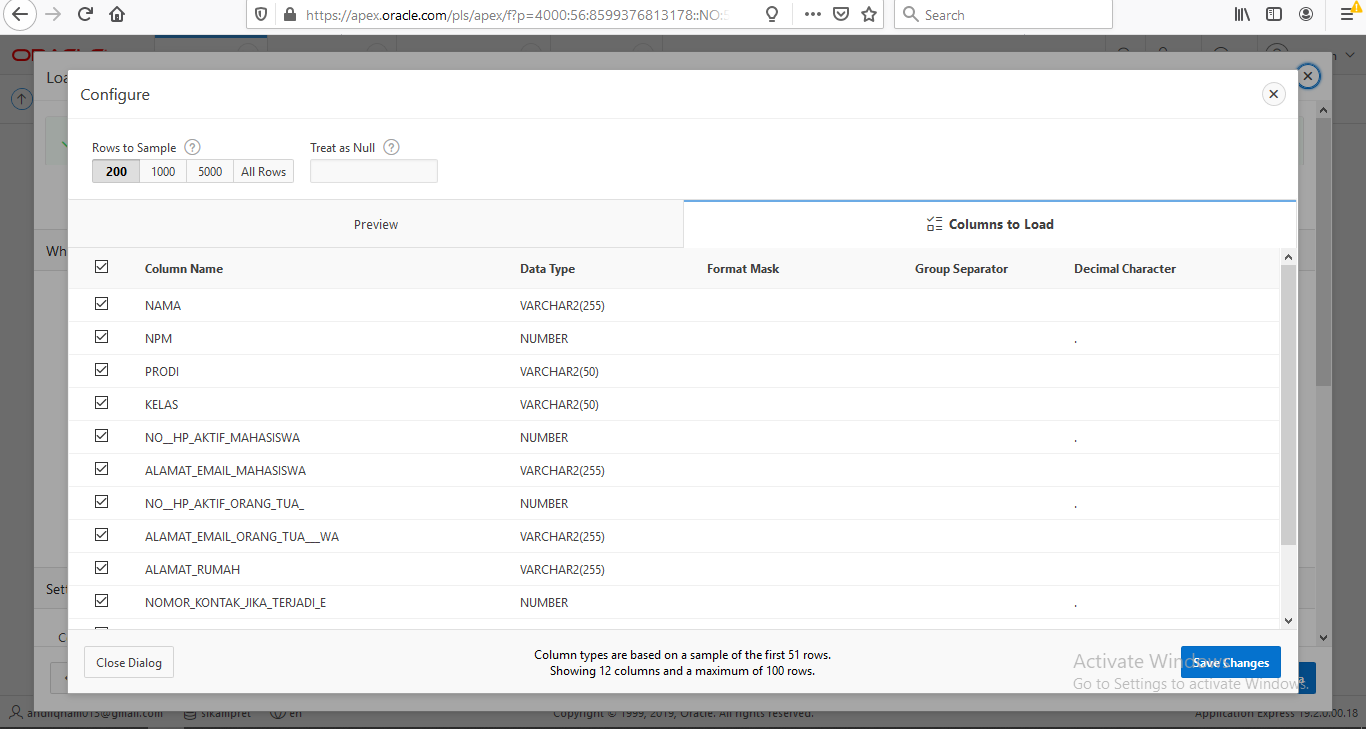
\includegraphics[width=.8\textwidth]{tb7.PNG}
\end{center}
    \item kita pilih save changes..untuk menyipan data yang telah diinput.
    \begin{center}
    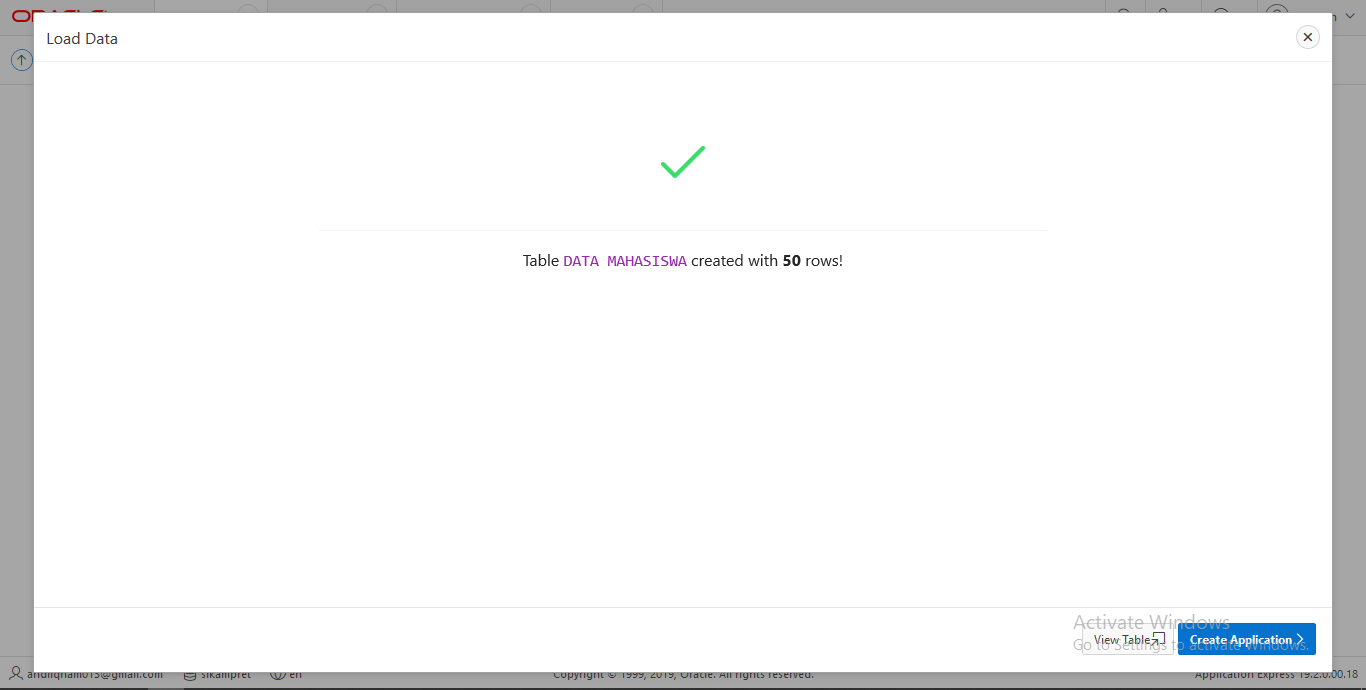
\includegraphics[width=.8\textwidth]{tb9.PNG}
\end{center}
    \item selanhutnya kita pilih create apllication,jika sudah tampil seperti ini ,kita isi title dengan nama MAHASISWA.
    \begin{center}
    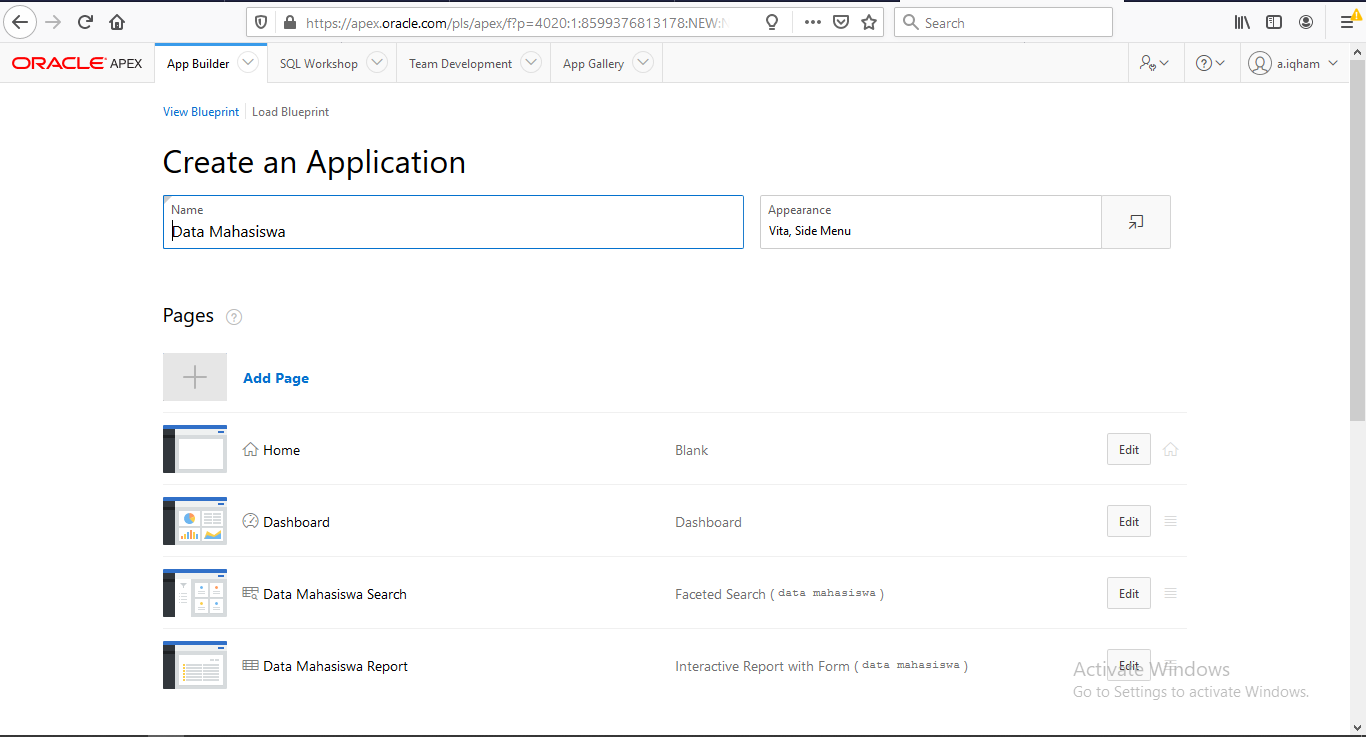
\includegraphics[width=.8\textwidth]{tb11.PNG}
\end{center}
    \item setelah itu kita kembali ke menu utama dan memilih check list all.
    \begin{center}
    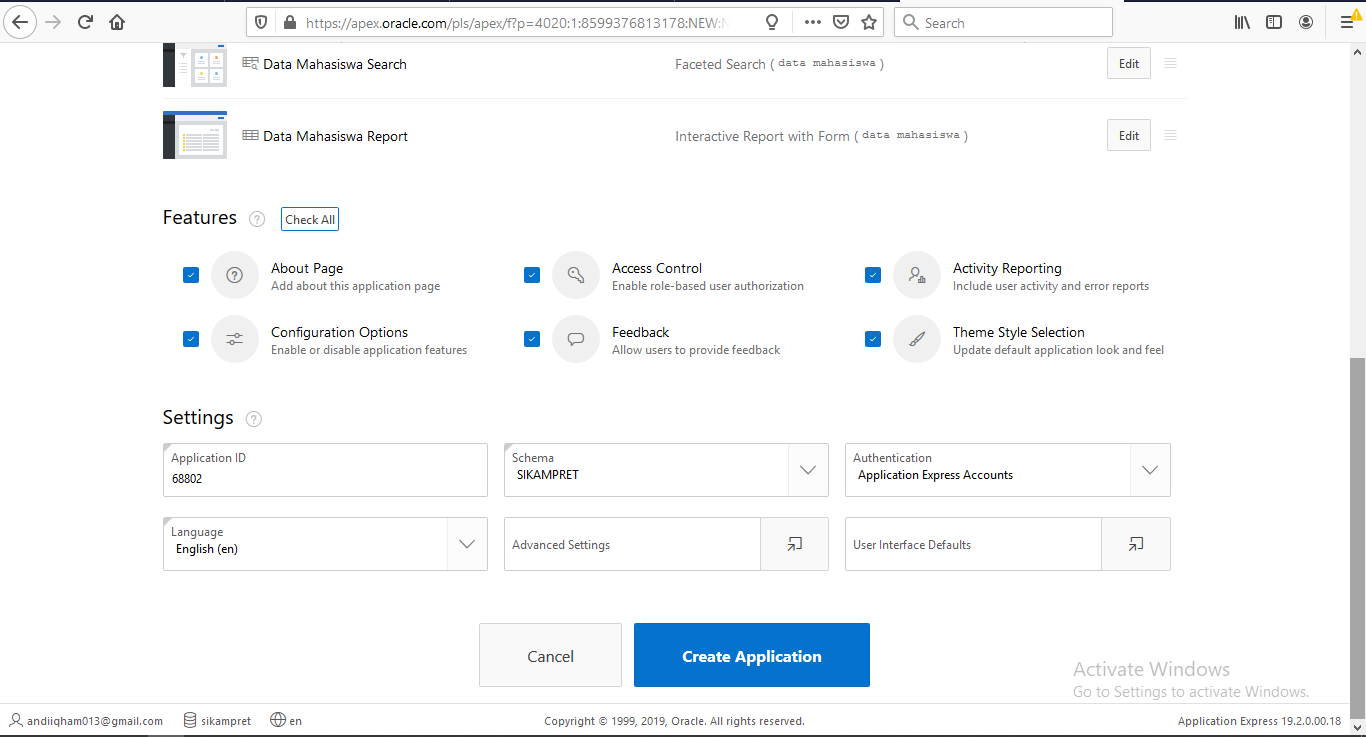
\includegraphics[width=.8\textwidth]{tb12.PNG}
\end{center}
    \item Jika sudah kita klik create application
    \begin{center}
    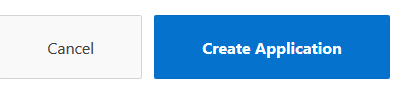
\includegraphics[width=.8\textwidth]{tb15.PNG}
\end{center}
    \item maka akan tampul menu seperti dibawah ini.
    \begin{center}
    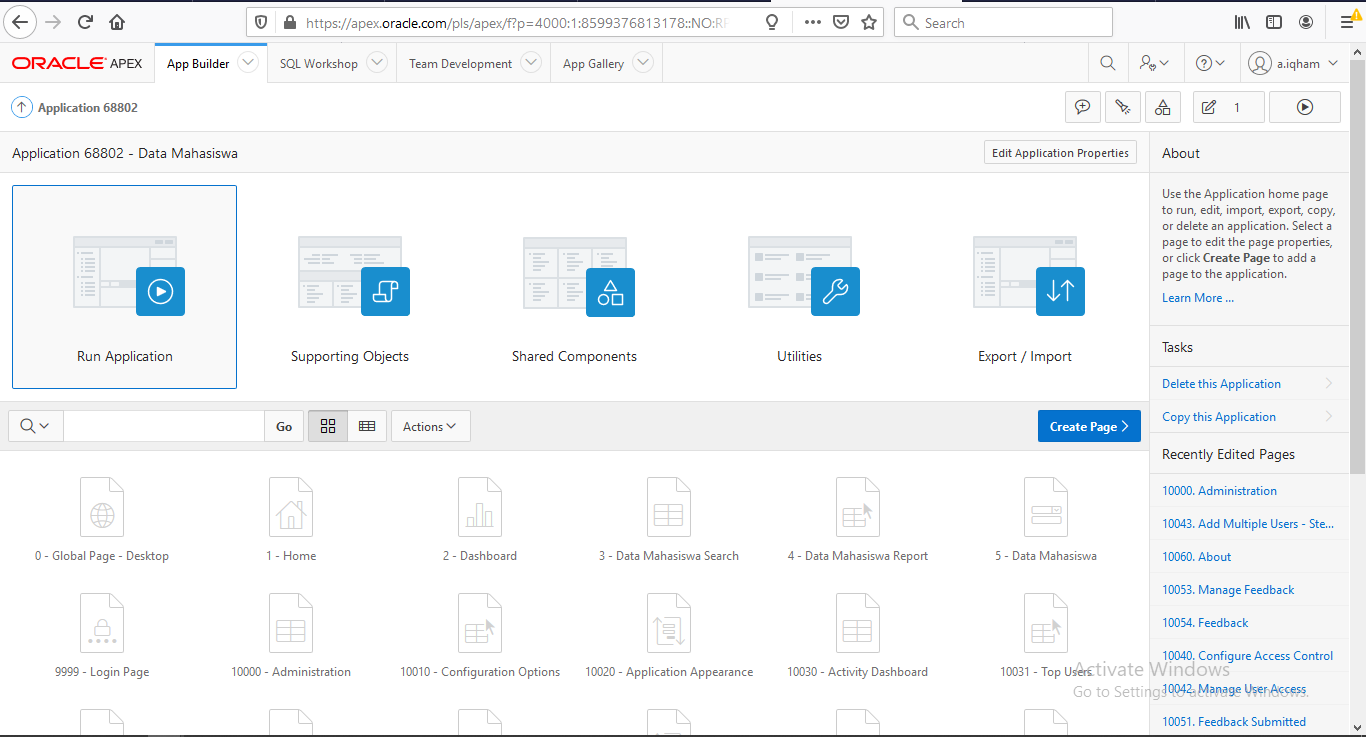
\includegraphics[width=.8\textwidth]{tb16.PNG}
\end{center}
    \item lalu kita pilih run application ini untuk menjalankan aplikasi
    \begin{center}
    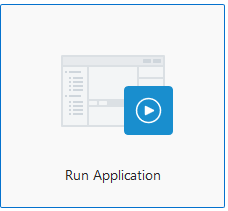
\includegraphics[width=.8\textwidth]{tb17.PNG}
\end{center}
    \item Setelah kita run application maka akan muncul form login.kita isi email dan password oracle apex.
    \begin{center}
    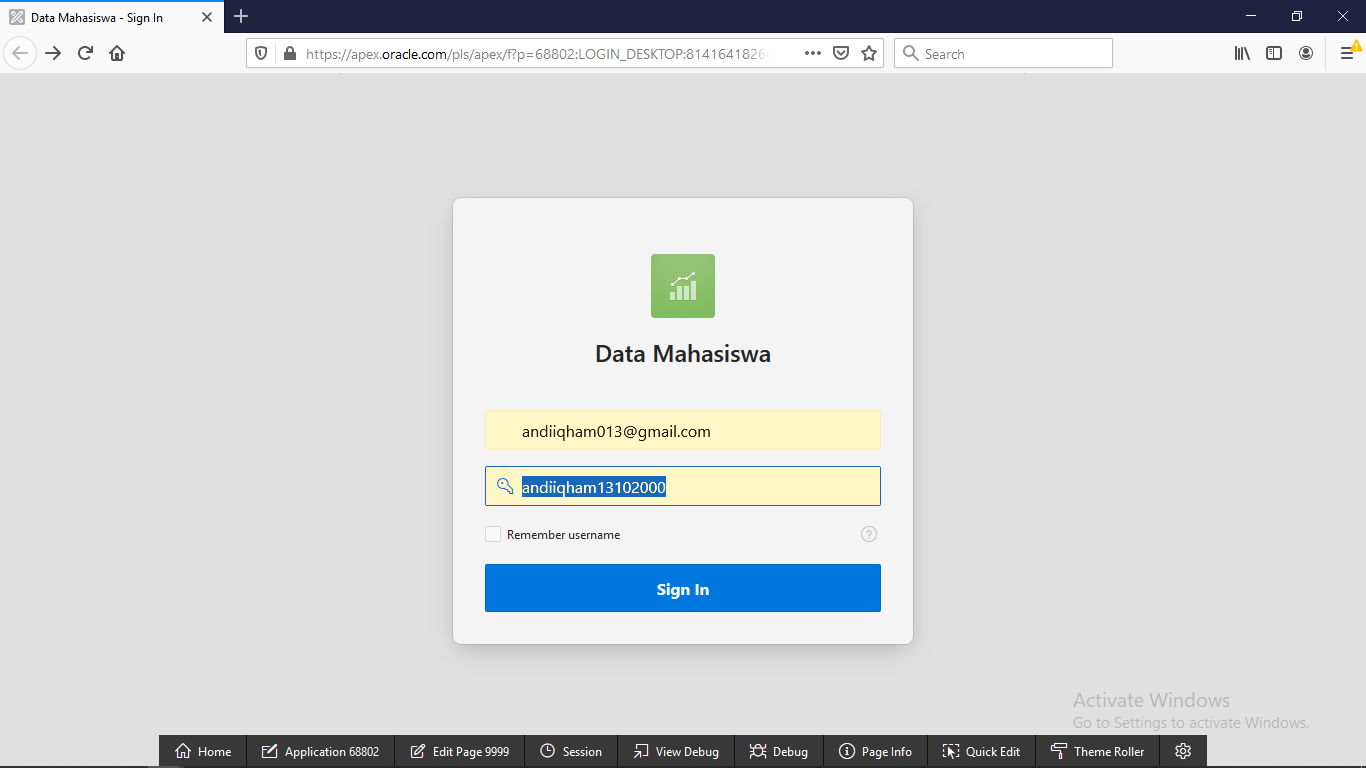
\includegraphics[width=.8\textwidth]{tb13.PNG}
\end{center}
    \item jika telah berhasil masuk,maka aplikasi kita telah jadi ..
    \begin{center}
    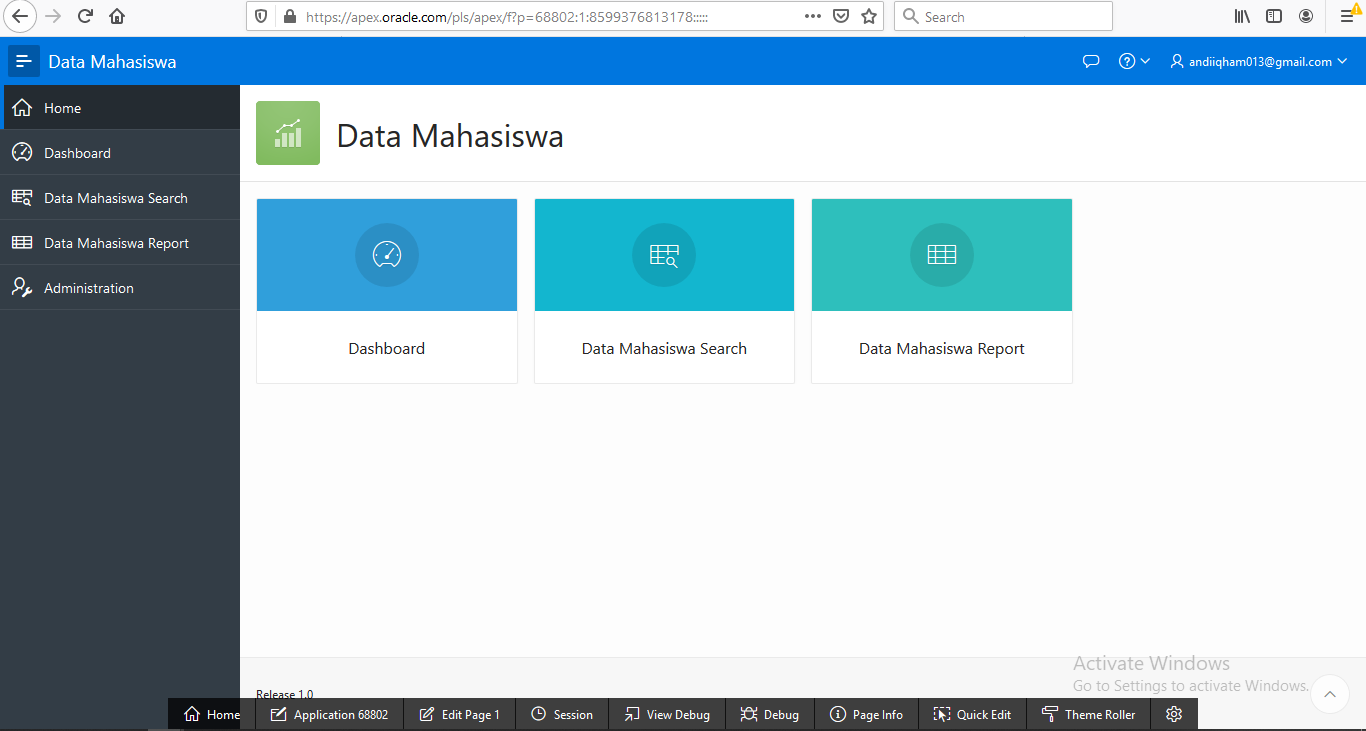
\includegraphics[width=.8\textwidth]{tb18.PNG}
\end{center}
    \item Dan data mahasiswa yang kita masukkan tadi secara otomatis akan ternormalisasi..
    \begin{center}
    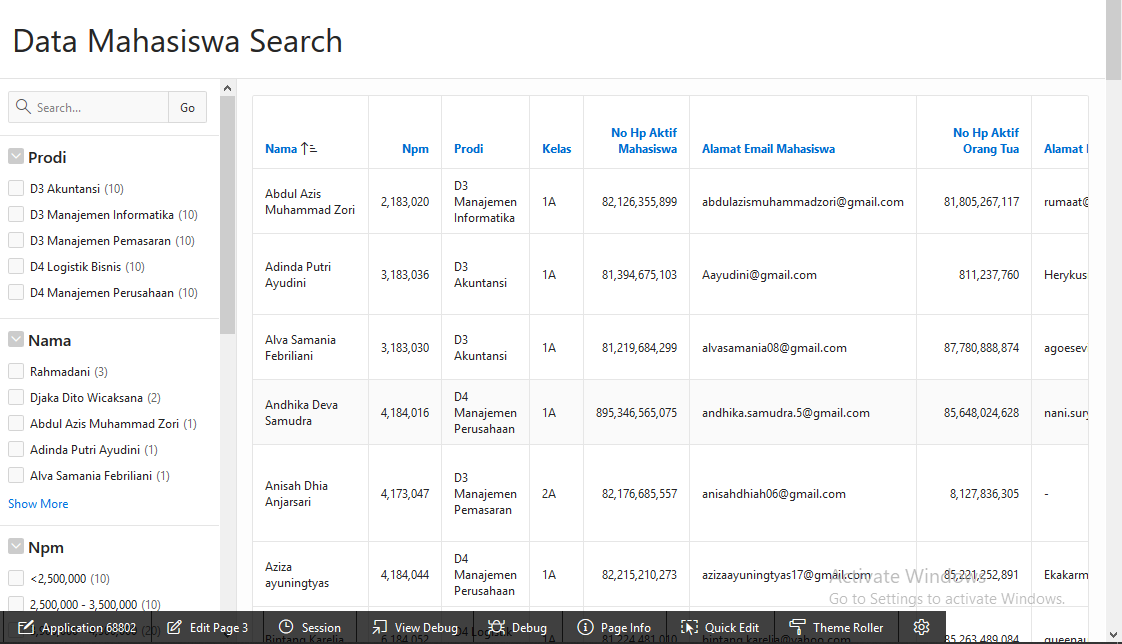
\includegraphics[width=.8\textwidth]{tb20.PNG}
\end{center}
\begin{center}
    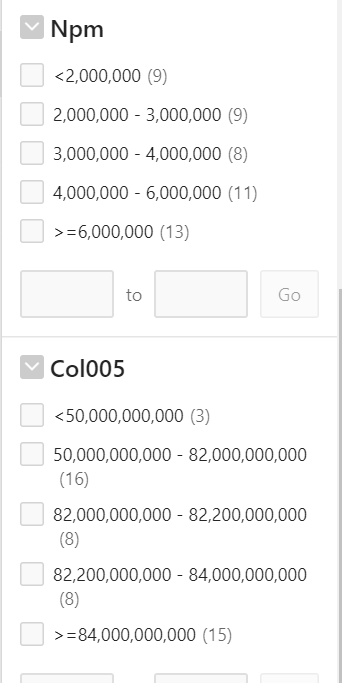
\includegraphics[width=.8\textwidth]{20.PNG}
\end{center}
    \item Dan aplikasi kita memiliki banyak pilihan menu.untuk lebih jelas silahkan lihat gambar di
   bawah ini.
   
   \begin{center}
    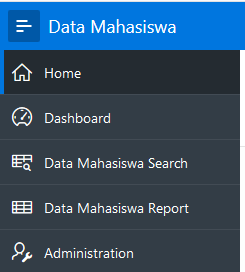
\includegraphics[width=.8\textwidth]{tb19.PNG}
\end{center}  
    \item dan itulah langkah-langkah membuat sistem informasi dengan menggunakan ORACLE APEX.
    \begin{center}
\end{center}
\end{enumerate}
\end{document}
